\documentclass[11pt,a4paper]{article}
\usepackage[T1]{fontenc}
\usepackage[utf8]{inputenc}
\usepackage{lmodern}
\usepackage[margin=2.5cm]{geometry}
\usepackage{amsmath,amssymb}
\usepackage{graphicx}
\usepackage{booktabs}
\usepackage{xcolor}
\usepackage[font=small,labelfont=bf]{caption}
\usepackage[colorlinks=true,linkcolor=blue!50!black,citecolor=blue!50!black,urlcolor=blue!50!black]{hyperref}

\newcommand{\dM}{\Delta M}
\newcommand{\tauE}{\tau_{\rm E}}
\newcommand{\Msun}{M_\odot}

\title{Can white holes merge?\\[4pt]
\large Eardley lifetimes from exact null-shell crossing and their consequences for white-hole binaries}
\author{Mustafa Karatüm\\[2pt]
\small Independent researcher \quad ORCID: \href{https://orcid.org/0009-0006-7053-2872}{0009-0006-7053-2872}}
\date{November 2026 \quad DOI: \href{https://doi.org/10.5281/zenodo.23855410}{10.5281/zenodo.23855410}}

\begin{document}
\maketitle

\begin{abstract}
White holes, the time reverses of black holes, are unstable to the accretion of even tiny amounts of matter (Eardley 1974). Using the exact thin-null-shell model of Barceló, Carballo-Rubio and Garay, we write the lifetime of an exploding white hole of mass $M$ exposed to an infalling shell of mass $\dM$ in closed form, $\tauE = 4M[\ln(M/\dM) - 1 - \dM/M]$ ($G=c=1$), give the crossing radius through the Lambert $W$ function, and show that the energy escaping from the explosion is exactly $M_\infty = M - \dM/w$, which for $\dM \ll M$ follows the universal profile $M_\infty/M \simeq 1 - e^{(\Delta t-\tauE)/4M}$; the rest stays behind as a black-hole remnant. Taking the smallest perturbations that are physically available, the cosmic microwave background gives $\tauE \lesssim 250$--$410\,M$ for masses from $10\,\Msun$ to $6.5\times10^{9}\,\Msun$, and a single quantum the size of the hole gives the absolute bound $\tauE \lesssim 880\,M$. We then compare $\tauE$ with the gravitational-wave inspiral time of a binary. A white hole survives until merger only if the binary already has a separation $a \lesssim 6$--$10\,M$ when the white hole first becomes exposed, within the last few orbits before plunge. In a white-hole pair, the burst of the first explosion leaves the companion only $12$--$50$ of its own mass units to explode before it is sealed into a black hole, even from $a = 1000\,M$. Together with the time reverse of Hawking's no-bifurcation theorem, which forbids two white-hole horizons from merging into one, these estimates indicate that white-hole--white-hole and white-hole--black-hole collisions end, in every channel we can follow, either in explosions that leave black-hole remnants or in an ordinary black-hole--black-hole merger. The estimates rest on spherical symmetry and null shells and are not a substitute for numerical relativity. All numbers are reproduced by a short open script, and an interactive 3D visualisation accompanies the paper.
\end{abstract}

\section{Introduction}

The Schwarzschild solution maximally extended in Kruskal coordinates contains, next to the black-hole region, a white-hole region: a past event horizon that nothing can cross from outside and out of which matter and radiation can only emerge~\cite{HawkingEllis}. A white hole is therefore the exact time reverse of a black hole. Its exterior gravity is the same attractive Schwarzschild field, and recent work shows that even its accretion disk has the same structure as that of a black hole, so that only the light crossing the white-hole horizon distinguishes the two~\cite{Li2025}.

Eardley showed early on that white holes are violently unstable~\cite{Eardley1974}. Matter that falls towards a white hole cannot enter it. It piles up just outside the past horizon, where it is strongly blueshifted relative to the outgoing flow, and its gravity bends the outgoing light cones until the white hole is sealed inside a new black-hole horizon. The instability has been re-derived in many ways~\cite{BBP1993,OriPoisson1994,Blau1989}. Barceló, Carballo-Rubio and Garay recast it in an exact model built from two crossing null shells, using the Dray--'t Hooft--Redmount (DTR) relation~\cite{DrayTHooft1985,Redmount1985}, and drew the lesson that a white-hole explosion either happens quickly or not at all: ``no half measures''~\cite{BCG2016}. White holes have recently returned to the literature as possible end states of evaporating black holes~\cite{HaggardRovelli2015,Bianchi2018}, which makes their stability a practical question.

This paper asks a simple question that, to our knowledge, has not been treated quantitatively: what happens when two white holes, or a white hole and a black hole, approach each other in a binary? A full answer would need numerical relativity with white-hole initial data, which does not exist. What can be done exactly is to turn the Barceló--Carballo-Rubio--Garay construction into a closed-form white-hole lifetime $\tauE$ (Sec.~\ref{sec:lifetime}), bound it from above with the smallest perturbations nature provides (Sec.~\ref{sec:floor}), and compare it with the time a binary needs to merge (Sec.~\ref{sec:binary}). Section~\ref{sec:limits} lists the assumptions that limit these estimates, and Sec.~\ref{sec:sim} describes the companion visualisation. We use $G=c=1$ throughout and quote physical times through $GM/c^3$.

\section{Exact null-shell model}\label{sec:model}

Following Ref.~\cite{BCG2016}, take the geometry of a white hole of mass $M$ exploding at retarded time $u_{\rm out}$: the exact time reverse of a null shell of mass $M$ collapsing to a black hole. Outside the outgoing shell the metric is Schwarzschild with mass $M$, and inside it is flat. In the Schwarzschild region we use Kruskal--Szekeres null coordinates,
\begin{equation}
U = -e^{-u/4M},\qquad V = e^{v/4M},\qquad UV = \Big(1-\frac{r}{2M}\Big)\,e^{r/2M},
\label{eq:kruskal}
\end{equation}
with $u=t-r_*$, $v=t+r_*$ and $r_*=r+2M\ln(r/2M-1)$ (Eqs.~1--2 of Ref.~\cite{BCG2016}). The outgoing shell runs along $U = U_{\rm out}$.

Now let an ingoing null shell of mass $\dM$ fall in along $V=V_{\rm in}$. Where the two shells cross, at radius $r_c$, four regions meet: the mass-$M$ region below the crossing, the flat region inside both shells, the mass-$(M+\dM)$ region outside both, and the region between the shells after the crossing, whose mass we call $\overline{M}$. The DTR relation, which follows from continuity of the metric at the crossing~\cite{DrayTHooft1985,Redmount1985}, reads
\begin{equation}
\Big(1-\frac{2M}{r_c}\Big)\Big(1-\frac{2\overline M}{r_c}\Big) = 1\cdot\Big(1-\frac{2(M+\dM)}{r_c}\Big).
\label{eq:dtr}
\end{equation}
Writing $r_c = 2(M+\dM)+\Delta r$, Eq.~\eqref{eq:dtr} gives Eqs.~(4)--(5) of Ref.~\cite{BCG2016},
\begin{equation}
\overline{M} = \frac{M+\dM+\Delta r/2}{\dM+\Delta r/2}\,\dM, \qquad M_\infty = M+\dM-\overline{M},
\label{eq:Mbar}
\end{equation}
where $M_\infty$ is the energy carried to infinity by the outgoing shell. After the crossing the ingoing shell, now carrying $\overline M$, continues inwards through the flat interior and collapses, so even a successful explosion leaves a black hole of mass $\overline M$ behind (the centre panel of Fig.~1 in Ref.~\cite{BCG2016}). If the crossing happens at or inside the combined Schwarzschild radius, $r_c \le 2(M+\dM)$, the outgoing shell is trapped and a black hole of mass $M+\dM$ forms instead of the explosion. In Kruskal coordinates this is the condition $U_{\rm out} < U_h$ with $U_h = -(\dM/M)\,e^{1+\dM/M}/V_{\rm in}$ for the explosion to proceed (Eqs.~6--7 of Ref.~\cite{BCG2016}).

\section{Closed-form lifetime and the escape profile}\label{sec:lifetime}

Translate the Kruskal condition into the time coordinates of the mass-$M$ region. Define
\begin{equation}
\Delta t \equiv u_{\rm out} - v_{\rm in},
\end{equation}
the delay between the moment the perturbation falls in and the moment the white hole explodes. At the radius $r_0$ where $r_*(r_0)=0$, $r_0 = 2M[1+W(e^{-1})] \approx 2.557\,M$, $\Delta t$ is simply the Schwarzschild time between the ingoing shell passing inwards and the explosion passing outwards. At any other radius $R$ the two events are separated by $\Delta t + 2r_*(R)$.

\paragraph{Crossing radius.} Eq.~\eqref{eq:kruskal} at the crossing gives $(r_c/2M-1)\,e^{r_c/2M-1} = e^{-\Delta t/4M-1}$, so
\begin{equation}
r_c = 2M\big[1+w\big],\qquad w = W_0\!\big(e^{-\Delta t/4M-1}\big),
\label{eq:rc}
\end{equation}
with $W_0$ the principal branch of the Lambert $W$ function. In terms of $w$, Eq.~\eqref{eq:Mbar} simplifies to $\overline M = \dM\,(1+w)/w$.

\paragraph{Lifetime.} The explosion escapes if and only if $r_c > 2(M+\dM)$, i.e.\ $w > \dM/M$. Since $W_0$ is increasing, this is $e^{-\Delta t/4M-1} > (\dM/M)\,e^{\dM/M}$, or $\Delta t < \tauE$ with
\begin{equation}
\boxed{\;\tauE = 4M\Big[\ln\frac{M}{\dM} - 1 - \frac{\dM}{M}\Big]\;}
\label{eq:tau}
\end{equation}
This is exact within the model. It is the familiar logarithmic Eardley time scale, $\tauE \simeq 4M\ln(M/\dM)$, with its order-one corrections fixed. The factor $4M$ is the inverse surface gravity $1/\kappa$ of the horizon. For $\Delta t \gtrsim 4M$, Eq.~\eqref{eq:rc} gives $r_c - 2M \simeq 2M\,e^{-\Delta t/4M-1}$: every extra $4M$ of delay pushes the crossing a factor $e$ closer to the horizon, so every factor of $e$ in $M/\dM$ buys only $4M$ of lifetime.

\paragraph{No half measures.} In terms of $w$ the energy balance is exact and simple:
\begin{equation}
M_\infty = M - \frac{\dM}{w}, \qquad \overline{M} = \dM + \frac{\dM}{w}.
\label{eq:exact}
\end{equation}
For $\dM\ll M$ and $\Delta t \gtrsim 4M$, $W_0(x)\simeq x$ and $e^{-\tauE/4M-1}\simeq \dM/M$, so $w \simeq (\dM/M)\,e^{(\tauE-\Delta t)/4M}$ and
\begin{equation}
\frac{M_\infty}{M} \simeq 1 - e^{(\Delta t-\tauE)/4M} \qquad (\Delta t\le\tauE,\ \dM\ll M),
\label{eq:profile}
\end{equation}
with relative corrections of order $\dM/M$. The escaping energy is independent of $\dM$ once time is measured from $\tauE$ (Fig.~\ref{fig:escape}), and the black-hole remnant is $\overline M \simeq M e^{(\Delta t-\tauE)/4M}$. An explosion at $\Delta t \ll \tauE$ escapes essentially whole and leaves a remnant of only about $\dM$. Half of the energy is lost at $\Delta t = \tauE - 4M\ln 2 \approx \tauE - 2.8M$, a fraction $1/e$ at $\tauE - 4M$, and all of it at $\tauE$; the fall from $M_\infty \simeq M$ to zero takes about $10M$. This window is narrow compared with $\tauE$ itself, which is hundreds of $M$ (Sec.~\ref{sec:floor}). That is the quantitative form of the ``no half measures'' statement of Ref.~\cite{BCG2016}: apart from a window of a few $M$ just before the deadline, a white hole either explodes almost completely or does not explode at all.

\begin{figure}[t]
\centering
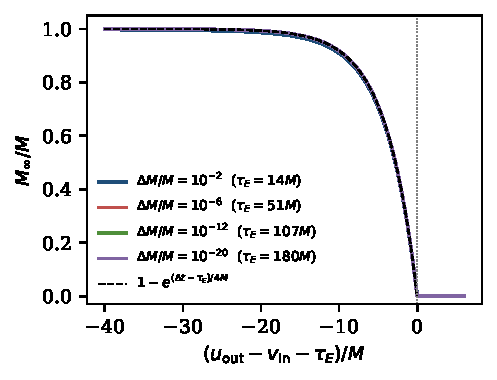
\includegraphics[width=0.48\textwidth]{figures/escape_fraction.pdf}\hfill
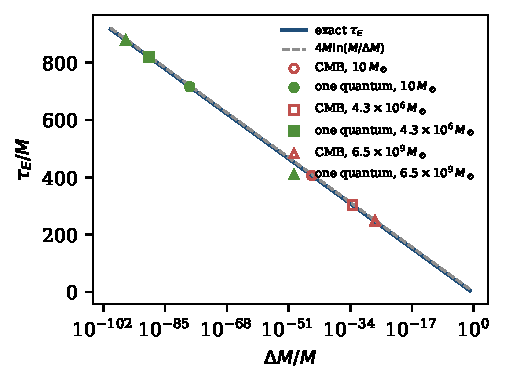
\includegraphics[width=0.48\textwidth]{figures/lifetime.pdf}
\caption{\emph{Left:} energy reaching infinity as a function of the explosion delay, from Eqs.~\eqref{eq:Mbar}--\eqref{eq:rc}, for four perturbation masses. Measured from $\tauE$ all curves coincide with the universal profile of Eq.~\eqref{eq:profile} (dashed). \emph{Right:} the lifetime of Eq.~\eqref{eq:tau} against $\dM/M$ over 99 decades, with the asymptotic form $4M\ln(M/\dM)$ (dashed) and the perturbation estimates of Table~\ref{tab:life}.}
\label{fig:escape}
\end{figure}

\section{How small can the perturbation be?}\label{sec:floor}

Because $\tauE$ grows only logarithmically, a white hole cannot buy a long life with a clean environment. We bound $\dM$ from below in two ways.

\paragraph{One quantum.} A perturbation that can be localised at the horizon must have a reduced wavelength no larger than the Schwarzschild radius $r_s=2M$. The smallest such energy is $\hbar c/r_s$, so $\dM_{\min} \simeq m_{\rm P}^2/2M$ with $m_{\rm P}=\sqrt{\hbar c/G}$. Then $\ln(M/\dM_{\min}) = 2\ln(M/m_{\rm P})+\ln 2$ and
\begin{equation}
\tauE^{\max} \simeq 4M\big[2\ln(M/m_{\rm P}) + \ln 2 - 1\big].
\end{equation}
This is a heuristic upper bound on the lifetime of any white hole that is not perfectly isolated. Quantum effects make white holes unstable in their own right~\cite{ZNS1974}, so an isolated white hole would not escape either. We do not use that result here.

\paragraph{The cosmic microwave background.} For $M \gtrsim \Msun$ the CMB wavelength is far smaller than $r_s$, and the hole captures CMB photons with the geometric-optics cross-section $\sigma = 27\pi M^2$. During one lifetime it collects $\dM = \sigma\,u_{\rm CMB}\,\tauE$, with $u_{\rm CMB}=aT^4$ at $T=2.7255$\,K. We solve this together with Eq.~\eqref{eq:tau} self-consistently. The CMB is a continuous flux rather than a single shell, so this treats the first $\tauE$'s worth of it as one shell, which is enough for a logarithm.

\begin{table}[t]
\centering
\caption{Eardley lifetimes from Eq.~\eqref{eq:tau}. $GM/c^3$ converts units of $M$ to seconds.}
\label{tab:life}
\small
\begin{tabular}{lccccccc}
\toprule
 & & \multicolumn{3}{c}{one quantum} & \multicolumn{3}{c}{CMB}\\
\cmidrule(lr){3-5}\cmidrule(lr){6-8}
mass & $GM/c^3$ [s] & $\dM/M$ & $\tauE/M$ & $\tauE$ [s] & $\dM/M$ & $\tauE/M$ & $\tauE$ [s]\\
\midrule
$10\,\Msun$ & $4.93\times10^{-5}$ & $6.0\times10^{-79}$ & 716 & $3.5\times10^{-2}$ & $2.6\times10^{-45}$ & 407 & $2.0\times10^{-2}$\\
$4.3\times10^{6}\,\Msun$ & $21.2$ & $3.2\times10^{-90}$ & 820 & $1.7\times10^{4}$ & $3.6\times10^{-34}$ & 304 & $6.4\times10^{3}$\\
$6.5\times10^{9}\,\Msun$ & $3.20\times10^{4}$ & $1.4\times10^{-96}$ & 879 & $2.8\times10^{7}$ & $6.6\times10^{-28}$ & 246 & $7.9\times10^{6}$\\
\bottomrule
\end{tabular}
\end{table}

Table~\ref{tab:life} gives the result for a stellar-mass hole and for holes with the masses of Sgr~A* and M87*. Both columns are upper bounds on the lifetime: any real environment adds gas, starlight or a companion, which only increases $\dM$ and shortens $\tauE$. With the CMB alone, $\tauE \lesssim 250$--$410\,M$ across nine decades of mass, and the absolute one-quantum bound is $\tauE \lesssim 880\,M$. A ten-solar-mass white hole therefore lives at most a few hundredths of a second after it is first touched by anything, and a supermassive one at most months.

\section{White holes in binaries}\label{sec:binary}

\paragraph{Exposure versus inspiral.} A white hole in a binary is never isolated: its companion, any gas in the system and the CMB all fall towards it. Its exposure starts when the binary forms, or when the white-hole phase begins, and it must explode within $\tauE$ of that moment or become a black hole. To reach merger as a white hole, the binary must coalesce faster than that. For a circular binary of total mass $M$, separation $a$ and symmetric mass ratio $\eta = m_1m_2/M^2$, the gravitational-wave inspiral time is~\cite{Peters1964}
\begin{equation}
t_{\rm GW}(a) = \frac{5}{256}\,\frac{a^4}{\eta M^3}.
\end{equation}
Setting $t_{\rm GW}(a_{\rm crit}) = \tauE$ gives the largest separation from which a white hole can still arrive at merger:
\begin{equation}
a_{\rm crit} = \Big(\frac{256}{5}\,\eta M^3\,\tauE\Big)^{1/4}.
\end{equation}
Table~\ref{tab:binary} and Fig.~\ref{fig:binary} show that $a_{\rm crit} \approx 5.7$--$10.3\,M$ for the whole range of $\tauE$ in Table~\ref{tab:life}. Integrating the Peters decay from $a_{\rm crit}$ down to the innermost stable circular orbit of a test particle at $6M$ gives between about one orbit ($\tauE=246M$, $q=1$) and five orbits ($\tauE=879M$). For $q=1/10$ and the CMB lifetime, $a_{\rm crit}=5.7M$ already lies inside $6M$, where a circular inspiral no longer describes the motion, so the white hole would have to be exposed during the plunge itself. For comparison, an equal-mass binary at $a=20\,M$ needs $1.25\times10^4\,M$ to merge, and at $a=100\,M$ it needs $7.8\times10^6\,M$. A white hole can only take part in a merger if it is born, or first exposed, already within the last few orbits.

\begin{table}[t]
\centering
\begin{minipage}{0.47\textwidth}
\centering
\caption{Critical separation $a_{\rm crit}$ for the shortest and longest $\tauE$ of Table~\ref{tab:life}.}
\label{tab:binary}
\small
\begin{tabular}{lccc}
\toprule
$q=m_2/m_1$ & $\eta$ & \multicolumn{2}{c}{$a_{\rm crit}/M$}\\
\cmidrule(lr){3-4}
 & & $\tauE=246M$ & $\tauE=879M$\\
\midrule
1 & 0.250 & 7.5 & 10.3\\
1/2 & 0.222 & 7.3 & 10.0\\
1/10 & 0.083 & 5.7 & 7.8\\
\bottomrule
\end{tabular}
\end{minipage}\hfill
\begin{minipage}{0.47\textwidth}
\centering
\caption{The first explosion in an equal-mass white-hole pair seals the companion ($m_1=m_2=M/2$).}
\label{tab:domino}
\small
\begin{tabular}{cccc}
\toprule
$a/M$ & captured & $\dM/m_2$ & $\tauE/m_2$\\
\midrule
10 & $1.7\times10^{-2}$ & $1.7\times10^{-2}$ & 12\\
20 & $4.2\times10^{-3}$ & $4.2\times10^{-3}$ & 18\\
100 & $1.7\times10^{-4}$ & $1.7\times10^{-4}$ & 31\\
1000 & $1.7\times10^{-6}$ & $1.7\times10^{-6}$ & 49\\
\bottomrule
\end{tabular}
\end{minipage}
\end{table}

\begin{figure}[t]
\centering
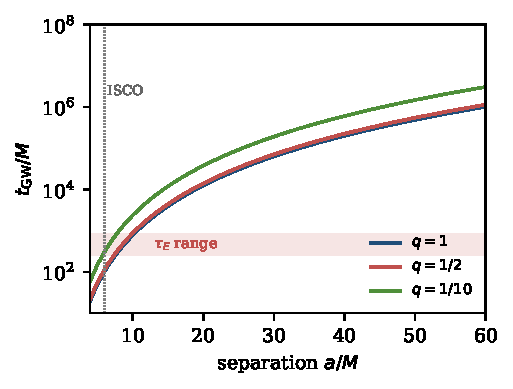
\includegraphics[width=0.55\textwidth]{figures/binary.pdf}
\caption{Gravitational-wave inspiral time against separation for three mass ratios. The shaded band is the range of white-hole lifetimes in Table~\ref{tab:life}. A white hole reaches merger only where the curves dip into the band, at $a\lesssim10\,M$. The dotted line marks the innermost stable circular orbit of a test particle, $6M$.}
\label{fig:binary}
\end{figure}

\paragraph{The domino effect.} Suppose the first white hole of a pair does explode in time. Its ejecta are a huge perturbation for its partner. Treating the burst as isotropic and taking all of $m_1$ as ejecta, the partner of mass $m_2$ at distance $a$ captures a fraction $27m_2^2/4a^2$ of it, giving $\dM/m_2 = 27 m_1 m_2/4a^2$. Table~\ref{tab:domino} shows that for equal masses the partner then has only $12$--$50\,m_2$ after the ejecta arrive, from $a=10\,M$ out to $a=1000\,M$. It explodes within that time, almost simultaneously with its companion, or it is sealed into a black hole that swallows part of the ejecta. This is an order-of-magnitude estimate. The capture cross-section $27\pi m_2^2$ assumes rays from far away, which is rough at $a=10M$, and an explosion that loses part of its energy to its own remnant sends less than $m_1$. Because $\tauE$ depends on $\dM$ only through a logarithm, an error of a factor of 10 in the captured mass shifts these times by only $4m_2\ln10 \approx 9\,m_2$.

\paragraph{No white-hole merger.} Even two white holes that reach contact cannot become one white hole. Hawking showed that, under the null energy condition and future asymptotic predictability (cosmic censorship), the total area of black-hole event horizons cannot decrease~\cite{Hawking1971} and that black holes can merge but never bifurcate~\cite{Hawking1972,HawkingEllis}. The ban on a white-hole merger comes from the second statement. Run backwards in time, it says that one white hole can split into two but two white holes cannot merge into one. The area law alone would not be enough: its time reverse only says that white-hole horizon area cannot increase, which a merger with $A_f \le A_1 + A_2$ would respect. The time-reversed theorems need the time-reversed hypotheses, namely the null energy condition and past asymptotic predictability. Ordinary cosmic censorship fails for every white hole, whose past singularity is visible from future null infinity, so the statement is about the class of spacetimes that are the exact time reverses of well-behaved black-hole spacetimes. The area law for black holes has been tested with the gravitational-wave event GW150914~\cite{Isi2021}.

\paragraph{Outcomes.} Putting the pieces together gives the following channels.
\begin{itemize}
\item \emph{White hole + white hole.} (i) Both explode within $\tauE$, well before contact: two bursts, each leaving a black-hole remnant of mass $\overline M$ (Eq.~\ref{eq:exact}), which is only about $\dM$ if the explosion comes early. Whether the remnants stay bound and later merge, as ordinary black holes, depends on how much mass the bursts carry off. (ii) One explodes first: its ejecta give the partner only $12$--$50\,m_2$, within which it also explodes or else is sealed into a black hole that captures part of the ejecta. (iii) Neither explodes within $\tauE$: both are sealed into black holes, and the system continues as an ordinary black-hole binary that later merges with the usual gravitational-wave signal.
\item \emph{White hole + black hole.} The white hole explodes within $\tauE$, leaving its own small remnant, and part of its ejecta fall into the black hole. Otherwise it is sealed and the pair continues as a black-hole binary.
\item \emph{Contact between a white-hole horizon and another horizon} requires the white hole to be first exposed at $a \lesssim a_{\rm crit}$, within the last few orbits before plunge. Even then, two white-hole horizons cannot merge into one. We know of no exact or numerical solution describing a white-hole horizon meeting a black-hole horizon, and we do not speculate about one.
\end{itemize}
A direct consequence is that a compact-binary inspiral observed in gravitational waves would look like a black-hole binary even if one or both members had started as white holes. Combined with the result that white-hole accretion disks look like black-hole ones~\cite{Li2025}, this makes white holes in binaries essentially invisible as such.

\section{Limitations}\label{sec:limits}

These estimates are exact only inside the model behind Eq.~\eqref{eq:tau}: spherical symmetry, a non-rotating hole, classical general relativity and matter represented by thin null shells. Barceló et al.\ argue, citing work on massive (timelike) shells~\cite{Nunez1993}, that these simplifications do not change the conclusion, and the logarithmic time scale has been found in several independent treatments~\cite{BBP1993,OriPoisson1994,Blau1989}. The binary application goes further than the model, in three ways. First, a companion and its ejecta are not spherical shells around the white hole. We use the spherical lifetime as an order-of-magnitude estimate, which the logarithm makes forgiving: an error of a factor $10^{10}$ in $\dM$ changes $\tauE$ by only $92M$. Second, the Peters inspiral time is a leading-order post-Newtonian result and is not accurate near $a\sim6$--$10\,M$, where higher-order effects shorten the time left to merger. Because $t_{\rm GW}\propto a^4$, an error of a factor of 2 in $t_{\rm GW}$ moves $a_{\rm crit}$ by only $2^{1/4}-1\approx19\%$, which keeps the white hole within the last few orbits. Third, the one-quantum bound and the CMB estimate are heuristic, and quantum effects of the kind that turn black holes into white holes~\cite{HaggardRovelli2015,Bianchi2018} lie outside the model. Rotating white holes, charged white holes and white holes formed in a binary already inside $a_{\rm crit}$ are left open.

\section{Companion visualisation}\label{sec:sim}

The paper comes with an interactive 3D visualisation that runs in a web browser (Fig.~\ref{fig:sim}). Besides an isolated white hole, it has collision modes for a white-hole pair and for a white hole with a black hole. The time at which each white hole is sealed into a black hole is taken from Eq.~\eqref{eq:tau}, and if the first white hole is set to explode earlier, its partner's deadline is shortened as in Table~\ref{tab:domino}. The orbit is a Newtonian circle shrinking at the Peters rate. The remnant of an early explosion, about $\dM$, is not drawn, and the visuals (particle outflows, glows, jets, lensing) are illustrative and are not part of the analysis.

\begin{figure}[t]
\centering
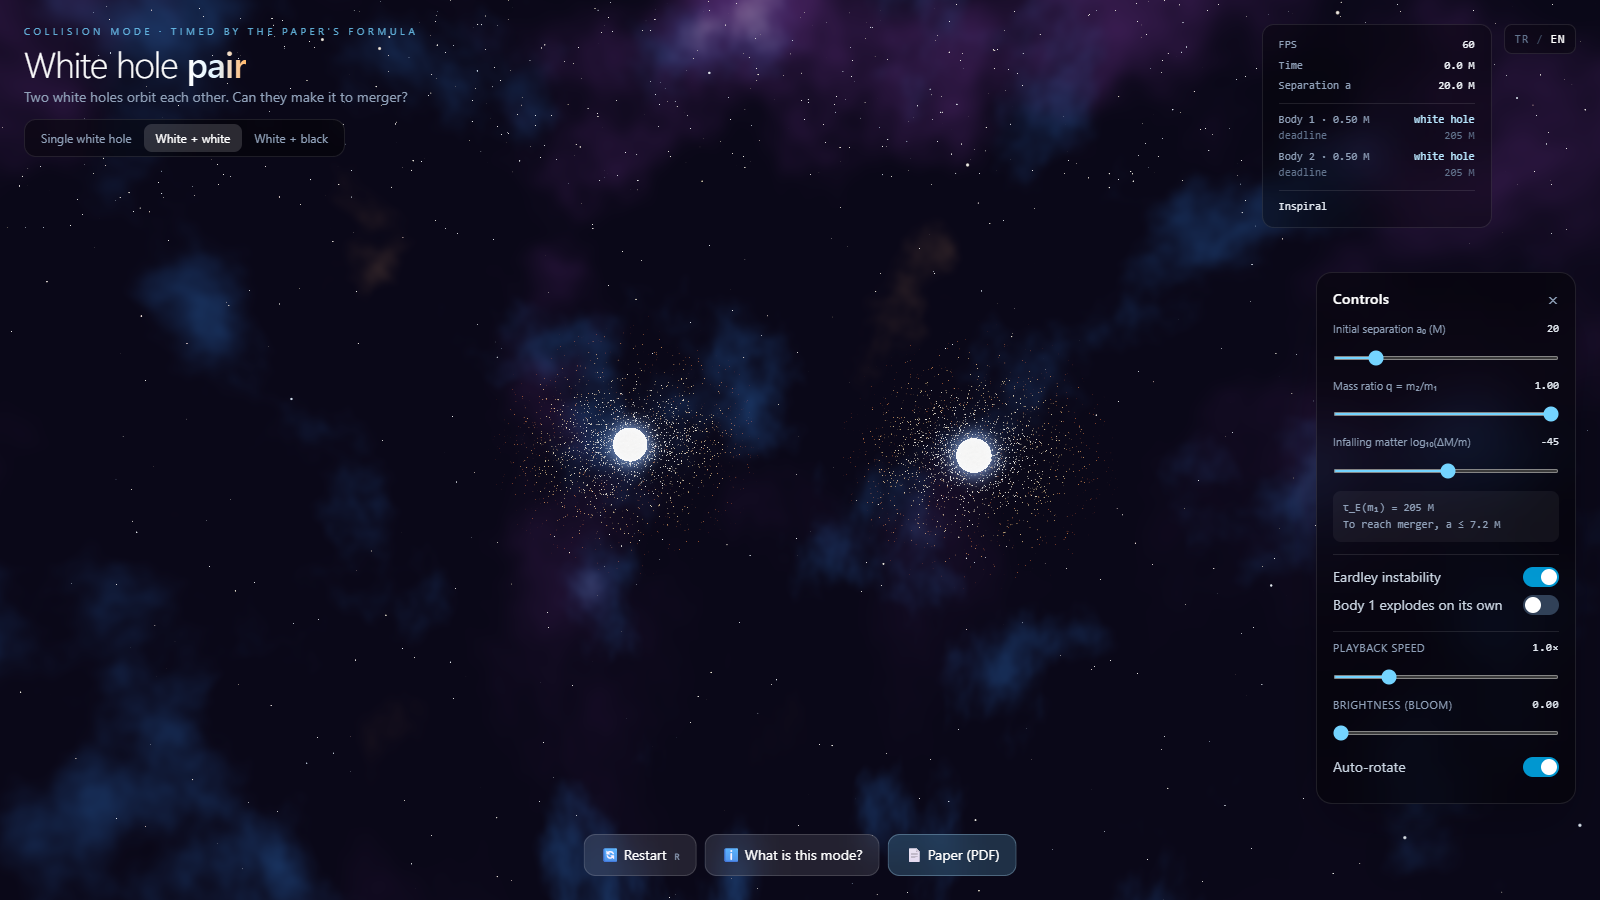
\includegraphics[width=0.49\textwidth]{../screenshots/wh-wh.png}\hfill
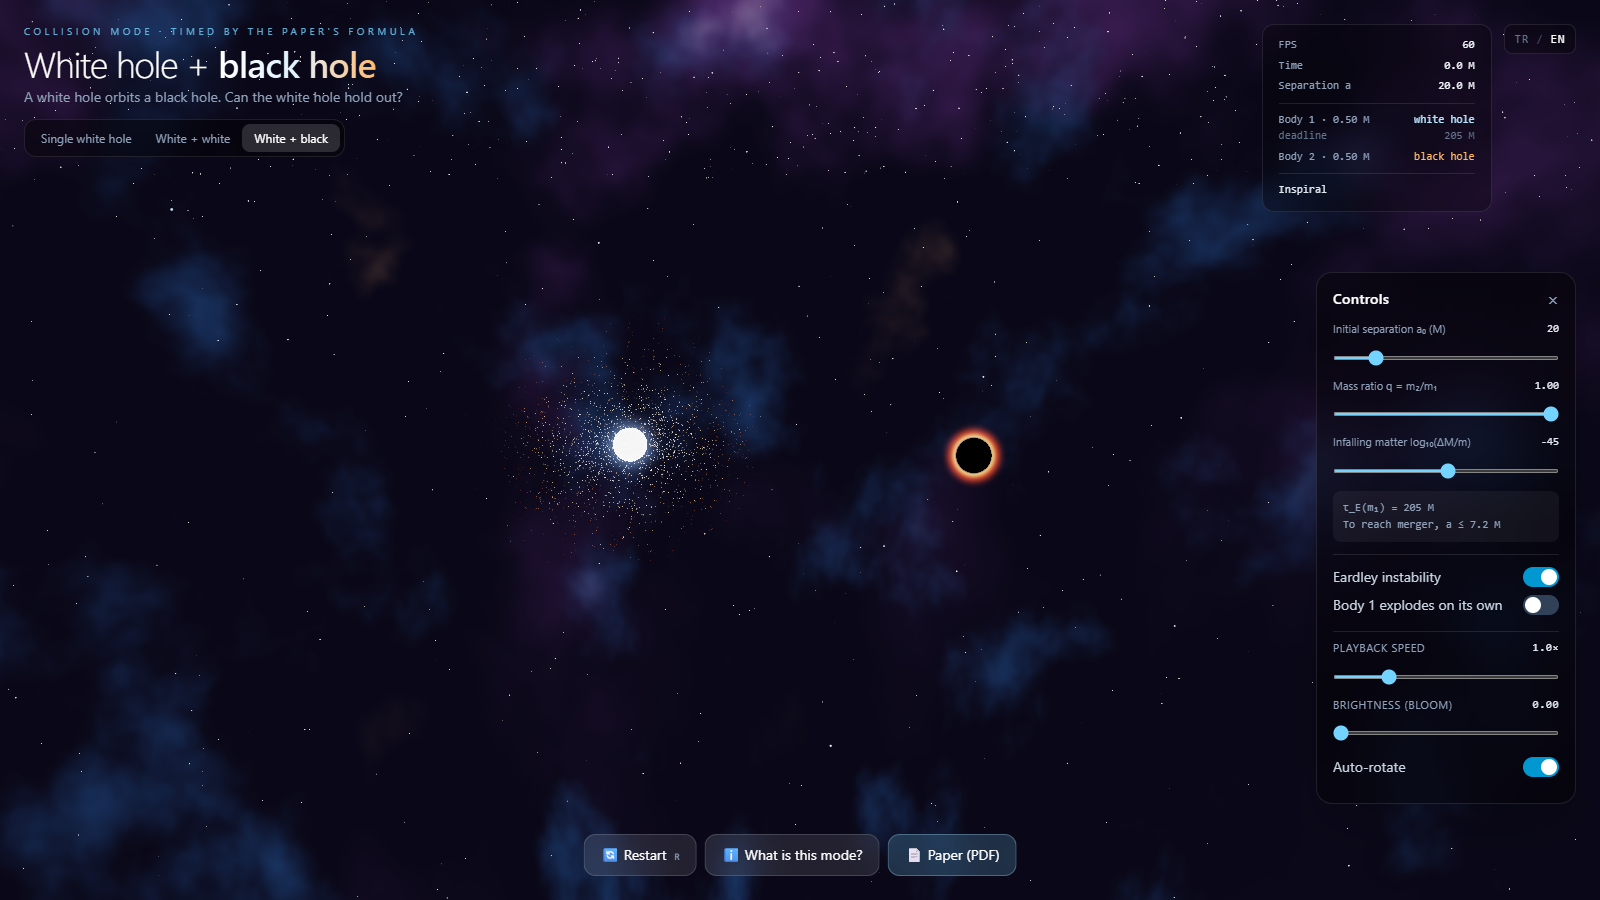
\includegraphics[width=0.49\textwidth]{../screenshots/wh-bh.png}
\caption{The collision modes of the companion visualisation: a white-hole pair (left) and a white hole orbiting a black hole (right). The panel shows the sealing time $\tauE$ of Eq.~\eqref{eq:tau} for the chosen $\dM$ and the separation $a_{\rm crit}$ from which the white hole could still reach merger.}
\label{fig:sim}
\end{figure} All numbers, tables and figures in this paper are produced by the script \texttt{paper/compute.py} in the same repository, which also checks the threshold condition, the DTR identity to $10^{-12}$ and the universal profile of Eq.~\eqref{eq:profile} against the exact expressions.

\section{Conclusion}

Within the exact null-shell model, the lifetime of a white hole exposed to a perturbation $\dM$ is $\tauE = 4M[\ln(M/\dM)-1-\dM/M]$, and its explosion energy falls off as $1-e^{(\Delta t-\tauE)/4M}$ as the deadline approaches, the rest staying behind as a black hole. The cosmic microwave background alone limits $\tauE$ to $\lesssim 250$--$410\,M$ for astrophysical masses, and a single quantum to $\lesssim 880\,M$. Gravitational-wave inspiral is far slower than this outside $a\approx6$--$10\,M$, a first explosion leaves the partner only tens of its mass units, and the time-reversed no-bifurcation theorem forbids a white-hole merger. Two white holes, or a white hole and a black hole, therefore do not collide as white holes. They explode first, leaving black-hole remnants, or they meet as black holes.

\section*{Code and data availability}
Source code of the analysis script and of the visualisation (MIT licence):\\
\url{https://github.com/pandakingpunc/white-hole-simulation}\\
Live visualisation:\\
\url{https://pandakingpunc.github.io/white-hole-simulation/}

\section*{Use of AI tools}
The analysis, the script, the figures and the text of this paper were prepared with the help of an AI assistant (Claude, by Anthropic, used through Claude Code). The author chose the research question, directed the work and is responsible for the content. All references were checked against their publishers' or arXiv records.

\begin{thebibliography}{99}
\bibitem{HawkingEllis} S.~W.~Hawking and G.~F.~R.~Ellis, \emph{The Large Scale Structure of Space-Time} (Cambridge University Press, 1973).
\bibitem{Li2025} L.~Li, Z.~Cao, Y.~Ling and X.~Wu, ``Accretion disk of a white hole,'' Chin.\ Phys.\ C \textbf{49}, 025109 (2025), \href{https://doi.org/10.1088/1674-1137/ad9899}{doi:10.1088/1674-1137/ad9899}.
\bibitem{Eardley1974} D.~M.~Eardley, ``Death of white holes in the early universe,'' Phys.\ Rev.\ Lett.\ \textbf{33}, 442 (1974), \href{https://doi.org/10.1103/PhysRevLett.33.442}{doi:10.1103/PhysRevLett.33.442}.
\bibitem{BBP1993} C.~Barrabès, P.~R.~Brady and E.~Poisson, ``Death of white holes,'' Phys.\ Rev.\ D \textbf{47}, 2383 (1993), \href{https://doi.org/10.1103/PhysRevD.47.2383}{doi:10.1103/PhysRevD.47.2383}.
\bibitem{OriPoisson1994} A.~Ori and E.~Poisson, ``Death of cosmological white holes,'' Phys.\ Rev.\ D \textbf{50}, 6150 (1994), \href{https://doi.org/10.1103/PhysRevD.50.6150}{doi:10.1103/PhysRevD.50.6150}.
\bibitem{Blau1989} S.~K.~Blau, ``'t Hooft--Dray geometries and the death of white holes,'' Phys.\ Rev.\ D \textbf{39}, 2901 (1989), \href{https://doi.org/10.1103/PhysRevD.39.2901}{doi:10.1103/PhysRevD.39.2901}.
\bibitem{DrayTHooft1985} T.~Dray and G.~'t~Hooft, ``The effect of spherical shells of matter on the Schwarzschild black hole,'' Commun.\ Math.\ Phys.\ \textbf{99}, 613 (1985), \href{https://doi.org/10.1007/BF01215912}{doi:10.1007/BF01215912}.
\bibitem{Redmount1985} I.~H.~Redmount, ``Blue-sheet instability of Schwarzschild wormholes,'' Prog.\ Theor.\ Phys.\ \textbf{73}, 1401 (1985), \href{https://doi.org/10.1143/PTP.73.1401}{doi:10.1143/PTP.73.1401}.
\bibitem{BCG2016} C.~Barceló, R.~Carballo-Rubio and L.~J.~Garay, ``Black holes turn white fast, otherwise stay black: no half measures,'' JHEP \textbf{01}, 157 (2016), \href{https://doi.org/10.1007/JHEP01(2016)157}{doi:10.1007/JHEP01(2016)157}, \href{https://arxiv.org/abs/1511.00633}{arXiv:1511.00633}.
\bibitem{HaggardRovelli2015} H.~M.~Haggard and C.~Rovelli, ``Quantum-gravity effects outside the horizon spark black to white hole tunneling,'' Phys.\ Rev.\ D \textbf{92}, 104020 (2015), \href{https://doi.org/10.1103/PhysRevD.92.104020}{doi:10.1103/PhysRevD.92.104020}.
\bibitem{Bianchi2018} E.~Bianchi, M.~Christodoulou, F.~D'Ambrosio, H.~M.~Haggard and C.~Rovelli, ``White holes as remnants: a surprising scenario for the end of a black hole,'' Class.\ Quantum Grav.\ \textbf{35}, 225003 (2018), \href{https://doi.org/10.1088/1361-6382/aae550}{doi:10.1088/1361-6382/aae550}.
\bibitem{ZNS1974} Ya.~B.~Zel'dovich, I.~D.~Novikov and A.~A.~Starobinsky, ``Quantum effects in white holes,'' Zh.\ Eksp.\ Teor.\ Fiz.\ \textbf{66}, 1897 (1974) [Sov.\ Phys.\ JETP \textbf{39}, 933 (1974)].
\bibitem{Peters1964} P.~C.~Peters, ``Gravitational radiation and the motion of two point masses,'' Phys.\ Rev.\ \textbf{136}, B1224 (1964), \href{https://doi.org/10.1103/PhysRev.136.B1224}{doi:10.1103/PhysRev.136.B1224}.
\bibitem{Hawking1971} S.~W.~Hawking, ``Gravitational radiation from colliding black holes,'' Phys.\ Rev.\ Lett.\ \textbf{26}, 1344 (1971), \href{https://doi.org/10.1103/PhysRevLett.26.1344}{doi:10.1103/PhysRevLett.26.1344}.
\bibitem{Hawking1972} S.~W.~Hawking, ``Black holes in general relativity,'' Commun.\ Math.\ Phys.\ \textbf{25}, 152 (1972), \href{https://doi.org/10.1007/BF01877517}{doi:10.1007/BF01877517}.
\bibitem{Isi2021} M.~Isi, W.~M.~Farr, M.~Giesler, M.~A.~Scheel and S.~A.~Teukolsky, ``Testing the black-hole area law with GW150914,'' Phys.\ Rev.\ Lett.\ \textbf{127}, 011103 (2021), \href{https://doi.org/10.1103/PhysRevLett.127.011103}{doi:10.1103/PhysRevLett.127.011103}.
\bibitem{Nunez1993} D.~Nunez, H.~P.~de~Oliveira and J.~Salim, ``Dynamics and collision of massive shells in curved backgrounds,'' Class.\ Quantum Grav.\ \textbf{10}, 1117 (1993), \href{https://doi.org/10.1088/0264-9381/10/6/008}{doi:10.1088/0264-9381/10/6/008}.
\end{thebibliography}

\end{document}
